\definecolor{deeppeach}{rgb}{1.0, 0.8, 0.64}

\newcommand{\mcell}[1]{\makecell{~\\[-0.75cm]\makebox[0pt]{#1}}}
\newcommand{\graytext}[1]{\color{gray} #1}
\newcommand{\bluetext}[1]{\bf \cellcolor{blue!15} #1}
\newcommand{\redtext}[1]{\bf \cellcolor{red!15} #1}

% Define a new pattern for spaced crosshatches
\pgfdeclarepatternformonly{my north east lines}{\pgfqpoint{-1pt}{-1pt}}{\pgfqpoint{10pt}{10pt}}{\pgfqpoint{6pt}{6pt}}%
{
  \pgfsetlinewidth{0.4pt}
  \pgfpathmoveto{\pgfqpoint{0pt}{0pt}}
  \pgfpathlineto{\pgfqpoint{3.1pt}{3.1pt}}
  \pgfusepath{stroke}
}

\newcommand{\crosshatchedcell}[1][9pt]{%
  \begin{tikzpicture}[baseline,overlay]
    \node[anchor=south west, inner sep=0pt, outer sep=0pt, minimum width=\linewidth + 1.5em, minimum height=0.67cm, pattern=my north east lines, pattern color=black!20] at (-0.2,0) {};
  \end{tikzpicture}%
}

% \newcommand{\crosshatchedcell}{%
%   \begin{tikzpicture}[baseline,overlay]
%     \node[anchor=south west, inner sep=0pt, outer sep=0pt, minimum width=\linewidth + 1.5em, minimum height=0.67cm, pattern=north east lines, pattern color=black!20] at (-0.2,0) {};
%   \end{tikzpicture}%
% }


\newcolumntype{M}[1]{>{\centering\arraybackslash}m{#1}}
\newcolumntype{G}{>{\columncolor{deeppeach!25}\centering\arraybackslash}m{0.08\linewidth}}
\newcolumntype{S}{>{\columncolor{gray!15}\centering\arraybackslash}M{0.10\linewidth}}
\newcommand\setrowheight{\rule{0pt}{0.67cm}}
\newcolumntype{g}{>{\columncolor{gray!25}\centering\arraybackslash}c}

\begin{table*}[h!]
    \centering
    \begin{tabular}{
        c
        g
        |S||
        G
        M{0.08\linewidth}
        M{0.08\linewidth}
        M{0.08\linewidth}
        ||G
        M{0.08\linewidth}
    }
        & \rotatebox{0}{\bf \large QOS metric} &
        \rotatebox{0}{\bf \large statistic} &
        \rotatebox{60}{\textit{baseline}} &
        \rotatebox{60}{\textit{$\Rightarrow$ multithread}} &
        \rotatebox{60}{\textit{$\Rightarrow$ intranode}} &
        \rotatebox{60}{\textit{+ compute}} &
        \rotatebox{60}{\textit{baseline}} &
        \rotatebox{60}{\textit{+ faulty hw}} \\
        \hline\hline
        \setrowheight
        \multirow[b]{4}{*}{\rotatebox[origin=c]{90}{Update Period}} &
            & \mcell{median} &
            \mcell{XX ns} &
            \bluetext{\mcell{$\Delta$-XX\%}} &
            \redtext{\mcell{$\Delta$\texttt{+}XX\%}} &
            \graytext{\mcell{$\Delta$+XX\%}} &
            \mcell{2.0 ms} &
            \graytext{\mcell{$\Delta$-0.5\%}} \\ \setrowheight

        &
            & \mcell{$\sim \mathrm{MAD}$} &
            \mcell{XX\%} &
            \graytext{\mcell{XX\%}} &
            \graytext{\mcell{XX\%}} &
            \redtext{\mcell{XX\%}} &
            \mcell{3.9\%} &
            \graytext{\mcell{4.0\%}} \\ \noalign{\vskip-0.7pt} \cdashline{3-9} \noalign{\vskip0.7pt}  \setrowheight

            &
                & \crosshatchedcell\mcell{mean} &
                \crosshatchedcell\mcell{XX ns} &
                \bluetext{\crosshatchedcell\mcell{$\Delta$-XX\%}} &
                \redtext{\crosshatchedcell\mcell{$\Delta$\texttt{+}XX\%}} &
                \graytext{\crosshatchedcell\mcell{$\Delta$+XX\%}} &
                \crosshatchedcell\mcell{2.0 ms} &
                \bluetext{\crosshatchedcell\mcell{$\Delta$-0.7\%*}}  \\ \setrowheight

        & \multirow[t]{4}{*}{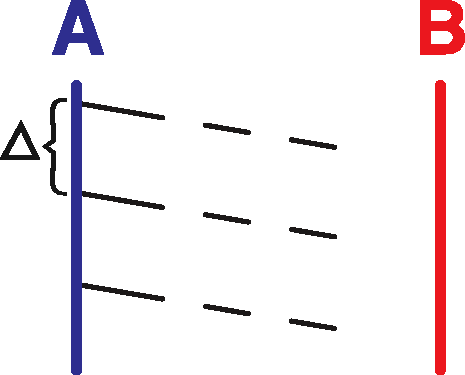
\includegraphics[height=2.8cm]{img/quality-of-service-metric-definitions/simstep-period-right.pdf}} &
            \crosshatchedcell\mcell{\% outliers} &
            \crosshatchedcell\mcell{XX\%} &
            \bluetext{\crosshatchedcell\mcell{XX\%}} &
            \graytext{\crosshatchedcell\mcell{XX\%}} &
            \graytext{\crosshatchedcell\mcell{XX\%}} &
            \crosshatchedcell\mcell{2.9\%} &
            \graytext{\crosshatchedcell\mcell{2.7\%}} \\
        \Xhline{4\arrayrulewidth}
        \setrowheight
        \multirow[t]{4}{*}{\rotatebox[origin=c]{90}{Walltime Latency~~~~~~~~~~~~~~~~~~~}} &
            & \mcell{median} &
            \mcell{XX ns} &
            \bluetext{\mcell{$\Delta$-XX\%}} &
            \redtext{\mcell{$\Delta$\texttt{+}XX\%}} &
            \graytext{\mcell{$\Delta$+XX\%}} &
            \mcell{2.3 ms} &
            \graytext{\mcell{$\Delta$-0.3\%}} \\ \setrowheight

        &
            & \mcell{$\sim \mathrm{MAD}$} &
            \mcell{XX\%} &
            \graytext{\mcell{XX\%}} &
            \graytext{\mcell{XX\%}} &
            \redtext{\mcell{XX\%}} &
            \mcell{12\%} &
            \graytext{\mcell{11\%}} \\ \noalign{\vskip-0.7pt} \cdashline{3-9} \noalign{\vskip0.7pt} \setrowheight

            &
                & \crosshatchedcell\mcell{mean} &
                \crosshatchedcell\mcell{XX ns} &
                \bluetext{\crosshatchedcell\mcell{$\Delta$-XX\%}} &
                \redtext{\crosshatchedcell\mcell{$\Delta$\texttt{+}XX\%}} &
                \graytext{\crosshatchedcell\mcell{$\Delta$+XX\%}} &
                \crosshatchedcell\mcell{2.4 ms} &
                \redtext{\crosshatchedcell\mcell{$\Delta$+446\%***}} \\ \setrowheight

        & \multirow[t]{4}{*}{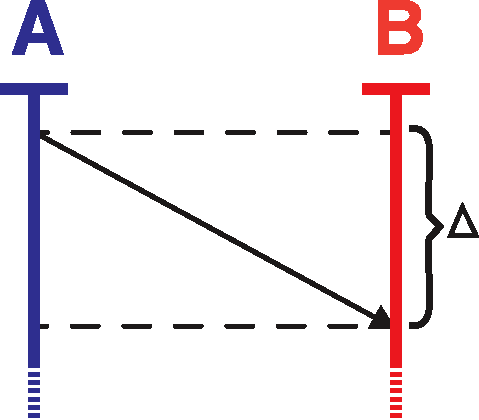
\includegraphics[height=2.8cm]{img/quality-of-service-metric-definitions/latency-right.pdf}} &
            \crosshatchedcell\mcell{\% outliers} &
            \crosshatchedcell\mcell{XX\%} &
            \bluetext{\crosshatchedcell\mcell{XX\%}} &
            \graytext{\crosshatchedcell\mcell{XX\%}} &
            \graytext{\crosshatchedcell\mcell{XX\%}} &
            \crosshatchedcell\mcell{1.8\%} &
            \graytext{\crosshatchedcell\mcell{2.1\%}} \\
        \Xhline{4\arrayrulewidth}
        \setrowheight
        \multirow[t]{4}{*}{\rotatebox[origin=c]{90}{Updates Latency~~~~~~~~~~~~~~~~~~~}} &
            & \mcell{median} &
            \mcell{XX updates} &
            \bluetext{\mcell{$\Delta$-XX\%}} &
            \redtext{\mcell{$\Delta$\texttt{+}XX\%}} &
            \graytext{\mcell{$\Delta$+XX\%}} &
            \mcell{1.2 updates} &
            \graytext{\mcell{$\Delta$+0.4\%}} \\ \setrowheight

        &
            & \mcell{$\sim \mathrm{MAD}$} &
            \mcell{XX\%} &
            \graytext{\mcell{XX\%}} &
            \graytext{\mcell{XX\%}} &
            \redtext{\mcell{XX\%}} &
            \mcell{12\%} &
            \redtext{\mcell{13\%*}} \\ \noalign{\vskip-0.7pt} \cdashline{3-9} \noalign{\vskip0.7pt} \setrowheight

            &
                & \crosshatchedcell\mcell{mean} &
                \crosshatchedcell\mcell{XX updates} &
                \bluetext{\crosshatchedcell\mcell{$\Delta$-XX\%}} &
                \redtext{\crosshatchedcell\mcell{$\Delta$\texttt{+}XX\%}} &
                \graytext{\crosshatchedcell\mcell{$\Delta$+XX\%}} &
                \crosshatchedcell\mcell{1.2 updates} &
                \redtext{\crosshatchedcell\mcell{$\Delta$+448\%***}} \\ \setrowheight

        & \multirow[t]{4}{*}{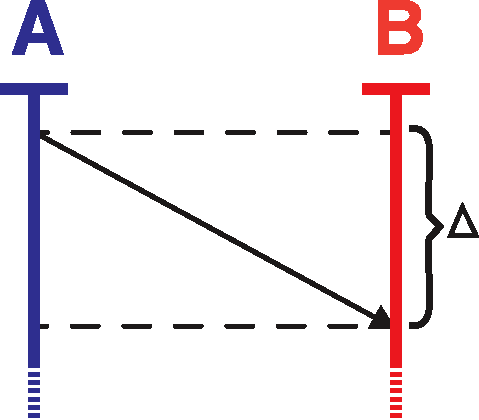
\includegraphics[height=2.8cm]{img/quality-of-service-metric-definitions/latency-right.pdf}} &
            \crosshatchedcell\mcell{\% outliers} &
            \crosshatchedcell\mcell{XX\%} &
            \bluetext{\crosshatchedcell\mcell{XX\%}} &
            \graytext{\crosshatchedcell\mcell{XX\%}} &
            \graytext{\crosshatchedcell\mcell{XX\%}} &
            \crosshatchedcell\mcell{1.9\%} &
            \redtext{\crosshatchedcell\mcell{2.3\%**}} \\
        \Xhline{4\arrayrulewidth}
        \setrowheight
        \multirow[b]{4}{*}{\rotatebox[origin=c]{90}{Bunching}} &
            & \mcell{median} &
            \mcell{XX} &
            \bluetext{\mcell{$\Delta$-XX\%}} &
            \redtext{\mcell{$\Delta$\texttt{+}XX\%}} &
            \graytext{\mcell{$\Delta$+XX\%}} &
            \mcell{0.32} &
            \graytext{\mcell{$\Delta$-0.5\%}} \\ \setrowheight

        &
            & \mcell{$\sim \mathrm{MAD}$} &
            \mcell{XX\%} &
            \graytext{\mcell{XX\%}} &
            \graytext{\mcell{XX\%}} &
            \redtext{\mcell{XX\%}} &
            \mcell{24\%} &
            \graytext{\mcell{24\%}} \\ \noalign{\vskip-0.7pt} \cdashline{3-9} \noalign{\vskip0.7pt} \setrowheight

            &
                & \crosshatchedcell\mcell{mean} &
                \crosshatchedcell\mcell{XX} &
                \bluetext{\crosshatchedcell\mcell{$\Delta$-XX\%}} &
                \redtext{\crosshatchedcell\mcell{$\Delta$\texttt{+}XX\%}} &
                \graytext{\crosshatchedcell\mcell{$\Delta$+XX\%}} &
                \crosshatchedcell\mcell{0.32} &
                \graytext{\crosshatchedcell\mcell{$\Delta$-0.6\%}} \\ \setrowheight

        & \multirow[t]{4}{*}{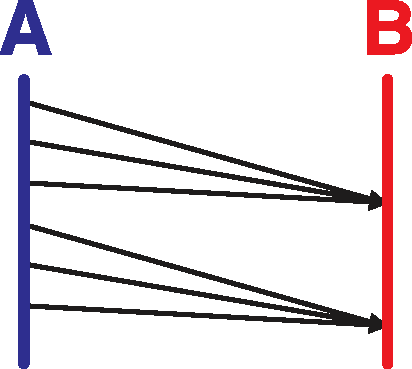
\includegraphics[height=2.8cm]{img/quality-of-service-metric-definitions/clumpiness-right.pdf}} &
            \crosshatchedcell\mcell{\% outliers} &
            \crosshatchedcell\mcell{XX\%} &
            \bluetext{\crosshatchedcell\mcell{XX\%}} &
            \graytext{\crosshatchedcell\mcell{XX\%}} &
            \graytext{\crosshatchedcell\mcell{XX\%}} &
            \crosshatchedcell\mcell{0.03\%} &
            \redtext{\crosshatchedcell\mcell{0.5\%***}} \\
        \Xhline{4\arrayrulewidth}
        \setrowheight
        \multirow[t]{4}{*}{\rotatebox[origin=c]{90}{Delivery Fail Rate~~~~~~~~~~~~~~~~~~}} &
            & \mcell{median} &
            \mcell{XX} &
            \bluetext{\mcell{$\Delta$-XX\%}} &
            \redtext{\mcell{$\Delta$\texttt{+}XX\%}} &
            \graytext{\mcell{$\Delta$+XX\%}} &
            \mcell{0} &
            \graytext{\mcell{0}} \\ \setrowheight

        &
            & \mcell{$\sim \mathrm{MAD}$} &
            \mcell{XX\%} &
            \graytext{\mcell{XX\%}} &
            \graytext{\mcell{XX\%}} &
            \redtext{\mcell{XX\%}} &
            \mcell{0\%} &
            \graytext{\mcell{0\%}} \\ \noalign{\vskip-0.7pt} \cdashline{3-9} \noalign{\vskip0.7pt} \setrowheight

            &
                & \crosshatchedcell\mcell{mean} &
                \crosshatchedcell\mcell{XX} &
                \bluetext{\crosshatchedcell\mcell{$\Delta$-XX\%}} &
                \redtext{\crosshatchedcell\mcell{$\Delta$\texttt{+}XX\%}} &
                \graytext{\crosshatchedcell\mcell{$\Delta$+XX\%}} &
                \crosshatchedcell\mcell{0} &
                \redtext{\crosshatchedcell\mcell{0.003\%**}} \\ \setrowheight

        & \multirow[t]{4}{*}{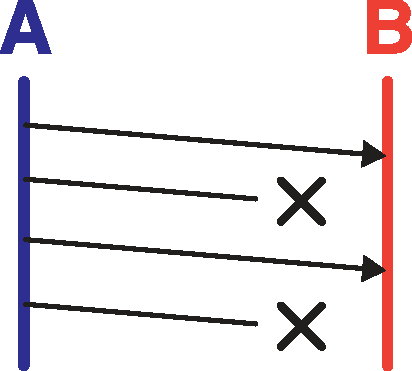
\includegraphics[height=2.8cm]{img/quality-of-service-metric-definitions/delivery-failure-rate-right.pdf}} &
            \crosshatchedcell\mcell{\% outliers} &
            \crosshatchedcell\mcell{XX\%} &
            \bluetext{\crosshatchedcell\mcell{XX\%}} &
            \graytext{\crosshatchedcell\mcell{XX\%}} &
            \graytext{\crosshatchedcell\mcell{XX\%}} &
            \crosshatchedcell\mcell{2.5\%} &
            \bluetext{\crosshatchedcell\mcell{0.7\%***}} \\
        \hline

    \end{tabular}
    \caption{%
      Best-effort communication quality of service (QOS) outcomes under experimental treatments, with 10 independent replicates per condition.
      Each QOS metric is described through four statistics.
      For each metric, the first two statistics (unhatched rows) describe typical QOS value and variance among typical QOS values.
      The second two statistics (hatched rows) describe outlier-inclusive QOS value and variance.
      Significantly degraded QOS outcomes are colored red, improved outcomes are blue, and baselines for comparison are peach.
      Significance denoted $* = p < 0.05$, $** = p < 0.005$, $*** = p < 0.0005$.
      QOS with no significant difference from baseline are grayed out.
      Statistic definitions are as follows, (1) median: median of replicate median observations, tested with quantile regression; (2) $\sim$MAD: median of relative median absolute deviance by replicate, tested with Mann-Whitney U; (3) mean: median of replicate observation means, tested with quantile regression; (4) percent outliers: percent outliers based on IQR definition, tested with chi-square contingency test.
      Values reported relative to baseline denoted $\Delta \texttt{+}x\%$ or $\Delta \texttt{-}x\%$.
    }
    \label{tab:categorical-composite}
\end{table*}
